% arara: clean: {
% arara: --> extensions:
% arara: --> ['aux', 'bbl', 'bcf', 'blg', 'idx', 'lof',
% arara: --> 'log', 'lol', 'mst', 'out', 'pdf', 'run.xml', 'toc']
% arara: --> }
% arara: lualatex: {
% arara: --> shell: yes,
% arara: --> draft: yes,
% arara: --> interaction: batchmode
% arara: --> }
% arara: biber
% arara: lualatex: {
% arara: --> shell: yes,
% arara: --> draft: yes,
% arara: --> interaction: batchmode
% arara: --> }
% arara: lualatex: {
% arara: --> shell: yes,
% arara: --> draft: yes,
% arara: --> interaction: batchmode
% arara: --> }
% arara: lualatex: {
% arara: --> shell: yes,
% arara: --> draft: no,
% arara: --> interaction: batchmode
% arara: --> }
% arara: clean: {
% arara: --> extensions:
% arara: --> ['aux', 'bbl', 'bcf', 'blg', 'idx', 'lof',
% arara: --> 'log', 'lol', 'mst', 'out', 'run.xml', 'toc']
% arara: --> }
\documentclass[
  aspectratio=1610,
  c,
  handout,
  8pt,
]{beamer}
\usepackage{diffcoeff}
\usepackage{minted}
\setminted[cpp]{highlightcolor=yellow!50!white}
\setminted[octave]{highlightcolor=yellow!50!white}
% \setminted[python]{highlightcolor=yellow!50!white}
% \setminted[toml]{highlightcolor=yellow!50!white}

\usefonttheme[onlymath]{serif}
\setbeamertemplate{navigation symbols}{}
\setbeamertemplate{headline}{}
\setbeamertemplate{footline}[frame number]{}
\setbeamertemplate{caption}[numbered]

\title{Introduction}
\institute{Universidad Nacional de Ingeniería}
\author{Carlos Aznarán}
\date{\today}

\begin{document}

\frontmatter
\maketitle
\chapter{Preface}

This document is for newcomers to MOLE (Mimetic Operator's
Library Enhanced) with a solid foundation in numerical analysis for
Partial Differential Equations (PDEs).
The library's algorithms are continuously evolving, with examples
implemented in
\href{https://octave.org}{GNU Octave}/\href{https://www.mathworks.com/products/matlab.html}{MATLAB},
\href{https://www.python.org}{Python} and
\href{https://isocpp.org}{C++} using the Armadillo sparse linear
algebra library.
Currently, these are only three language implementations available.
However, mastering this content will enable users to translate the
algorithms into other high-performance
scientific programming languages, such as
\href{https://julialang.org}{Julia},
\href{https://fortran-lang.org}{Fortran},
\href{https://www.rust-lang.org}{Rust} and
\href{https://www.open-std.org/jtc1/sc22/wg14}{C}.

The main goal of this manual is to provide clear explanations and
complete examples to help users understand the core
concepts and applications of the library.

We would like to thank Professor
\href{https://ctivitae.concytec.gob.pe/appDirectorioCTI/VerDatosInvestigador.do?id_investigador=45848}{Miguel Dumett}
of the Computational Science Research Center at San Diego State
University and the National University of Trujillo for organizing
MOLE courses.

\begin{figure}[ht!]
	\centering
	
\includegraphics[width=.32\paperwidth]{mole2024}\quad
	
\includegraphics[width=.32\paperwidth]{mole2025}
	\caption*{\bfseries Mimetic Methods courses in January and February 2024 and 2025.}
\end{figure}

\begin{flushright}
	Lima, Puno \hfill Carlos Aznarán \\[.5\baselineskip]

	March 2025 \hfill Adelaida Otazu
\end{flushright}

\tableofcontents
\listoflistings
% TODO: Agregar a la tabla de contenidos
% Octave/MATLAB scripts
% C++ scripts
% Python scripts

\mainmatter
\part{The Foundations of the Mimetic Finite Difference Operators 1D}

\chapter{Introduction and Objectives}

\chapter{Mimetic Operadors List}

\section{Divergence}

\section{Gradient}

\section{Interpolation from center to nodes}

\section{Interpolation from nodes to center}

\section{Laplacian}

\chapter{Numerical Methods for ODEs}

\todo{Only the methods used in the tutorials: Verlett, RK4, Explicit Euler}

\chapter{Numerical Solutions of Boundary Value Problems}

\chapter{Numerical Methods for PDEs}

\section{von Neumann Stability Criterion}

\section{Stability and Convergence Analysis}
\part{Numerical Exercises}

\chapter{Foo}

\section{Meeting MOLE}

The official website is \url{https://csrc-sdsu.github.io/mole}.
After skimming the description and reading the papers you will find out that this method never uses a ghost points.

\subsection{Create the staggered grid}

\section{Transport 1D}

\begin{equation*}
    \diffp{u}{t}+c\diffp{u}{x}=
    0.
\end{equation*}

\begin{listing}[ht!]
    \tiny
    \centering
    \pathinputminted[frame=single,framesep=10pt,linenos,firstline=9,lastline=35,highlightlines={9}]{cpp}{hyperbolic1D_upwind.cpp}
    \caption{Programa~\texttt{hyperbolic1Dupwind.cpp}}
    \label{code:hyperbolic1Dupwind.cpp}
\end{listing}

\section{Poisson 1D}

\begin{listing}[ht!]
    \tiny
    \centering
    \pathinputminted[frame=single,framesep=10pt,linenos,firstline=1,lastline=53,highlightlines={21,29}]{octave}{elliptic1D.m}
    \caption{Programa~\texttt{elliptic1D.m}}
    \label{code:elliptic1D.m}
\end{listing}

\begin{equation}\label{eq:poisson1drobindconditions}
    \left\{
    \begin{aligned}
        \diff[2]{u}{x}
         & =e^{x},
        \text{ para }x\in\left[0,1\right].     \\
        0
         & = u\left(0\right)-\diff{u}{x}[x=0]. \\
        2e
         & =u\left(1\right)+\diff{u}{x}[x=1].
    \end{aligned}
    \right.
\end{equation}

\begin{itemize}
    \item

          En la línea $1$ encontramos el
          \emph{shebang}\footnote{\url{https://en.wikipedia.org/wiki/Shebang_(Unix)}},
          esto permite ejecutar un script de Octave
          \mintinline{bash}|./elliptic1D.m| con la opción de modo de
          procesamiento por lotes (batch), para esto se necesita
          tener permisos de ejecución (por ejemplo,
          \mintinline{bash}|chmod +x elliptic1D.m|).

    \item

          En las líneas $2$ al $10$ tenemos un comentario sobre el
          programa de modo que ayude al codificador a obtener un
          contexto del problema a resolver.

    \item

          En la línea $12$, la función
          \href{https://docs.octave.org/v9.3.0/Manipulating-the-Load-Path.html#index-addpath}{\mintinline{octave}|addpath|}
          agrega el directorio
          \mintinline{octave}|"/usr/share/mole/matlab/"| a la ruta de
          búsqueda de la función.
          Allí se encuentran el conjunto de scripts Octave / MATLAB
          de la biblioteca MOLE.
          Vea el Programa~\ref{code:moledirectoriesoctave.txt}.

    \item

          En las líneas $14$ y $15$, se inicializan los identicadores
          \mintinline{octave}|west| (oeste, izquierda),
          \mintinline{octave}|east| (este, derecha) con los valores
          de $0$ y $1$, respectivamente, estos representan los
          valores de frontera del dominio espacial
          en~\eqref{eq:poisson1drobindconditions}.

    \item

          En la línea $21$, llamamos a la función
          \href{https://carlosal1015.github.io/mole_examples/api_docs/matlab/src/matlab/lap.html}{\mintinline{octave}|lap|},
          este genera un operador Laplaciano discreto extendido que
          requiere como argumentos obligatorios el orden de precisión
          \mintinline{octave}|k|, el número  de celdas
          \mintinline{octave}|m| y el tamaño de paso
          \mintinline{octave}|dx|.
          \begin{equation*}
              L=L^{\left(k\right)}=
              D^{\left(k\right)}
              G^{\left(k\right)}=
              DG.\qquad\qquad
              \left(
              \difc.L.{}{}=\nabla\cdot\nabla
              \right),
          \end{equation*}
          donde $D$ y $G$ son los operadores miméticos de divergencia
          y gradiente, respectivamente.
          Dado que
          \begin{math}
              D\in
              \mathbb{R}^{\left(m+2\right)\times\left(m+1\right)}
          \end{math}
          y
          \begin{math}
              G\in
              \mathbb{R}^{\left(m+1\right)\times\left(m+2\right)}
          \end{math},
          entonces
          \begin{math}
              L\in
              \mathbb{R}^{\left(m+2\right)\times\left(m+2\right)}
          \end{math}.

    \item

          En la línea $22$, con la función
          \href{https://docs.octave.org/v9.3.0/Figure-Properties.html#index-figure-visible}{\mintinline{octave}|figure|}
          desactivamos que se muestre la figura en la pantalla,
          preferimos solamente guardar la gráfica.

    \item

          En la línea $23$, con la función
          \href{https://docs.octave.org/latest/Information.html#index-spy}{\mintinline{octave}|spy|}
          graficamos (no se mostrará) el patrón de dispersidad de
          $L$.

          \begin{figure}[ht!]
              \centering
              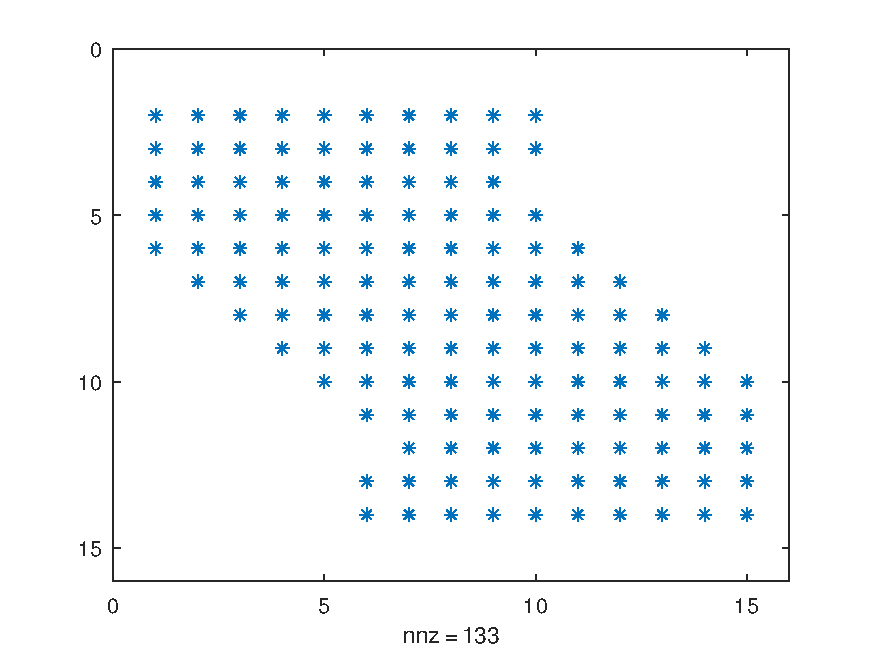
\includegraphics[width=.39\paperwidth]{../examples/octave/elliptic1Dsparsebefore.pdf}
              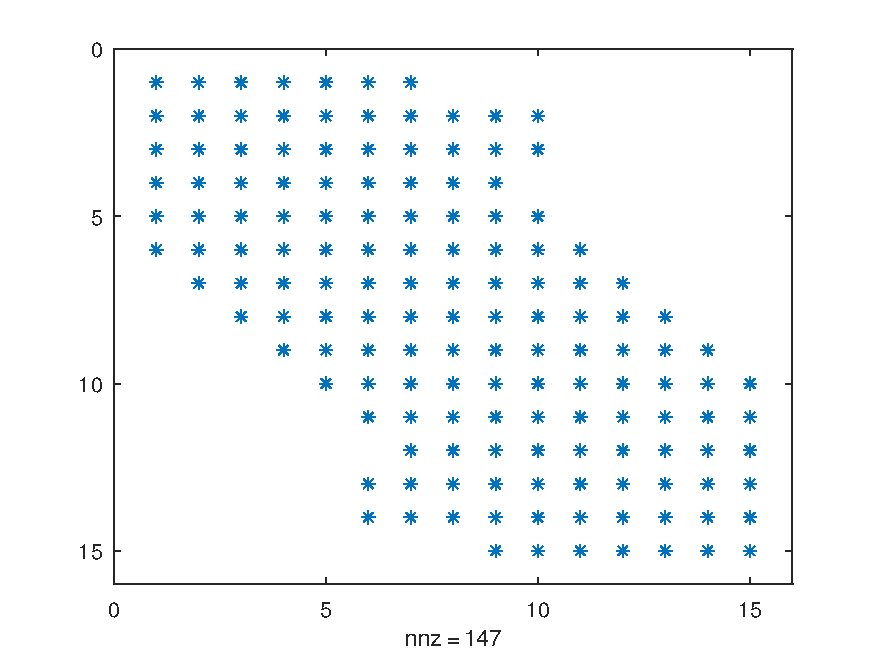
\includegraphics[width=.39\paperwidth]{../examples/octave/elliptic1Dsparseafter.pdf}
              \caption{Izquierda: Representación dispersa de $L$ hasta la línea
                  21.
                  La primera y la última fila son vectores de ceros.
                  Derecha: Representación dispersa de $L$ hasta la línea 29.
                  La matriz $L\in\mathbb{R}^{15\times 15}$.}
          \end{figure}

    \item

          En la línea $24$, con la función
          \href{https://docs.octave.org/latest/Printing-and-Saving-Plots.html}{\mintinline{octave}|saveas|}
          guardamos esta gráfica en formato PDF y recortado.

    \item

          En la línea $29$, llamamos a la función
          \href{https://carlosal1015.github.io/mole_examples/api_docs/matlab/src/matlab/robinBC.html}{\mintinline{octave}|robinBC|},
          este requiere como argumentos obligatorios el orden de
          precisión \mintinline{octave}|k|, el número  de celdas
          \mintinline{octave}|m|, el tamaño de paso
          \mintinline{octave}|dx|, el coeficiente Dirichlet
          \mintinline{octave}|a| y el coeficiente Neumann
          \mintinline{octave}|b|.
          Esta función devuelve una matriz en
          \begin{math}
              \mathbb{R}^{\left(m+2\right)\times\left(m+2\right)}
          \end{math}.
          Actualizamos la matriz \mintinline{octave}|L| según el
          Algoritmo~\ref{algo:updateL}.

          \begin{algorithm}[H]
              \caption{Actualizaciones del operador Laplaciano discreto extendido.}\label{algo:updateL}
              $A\leftarrow L$\;
              $F\leftarrow f$\;
              $A\leftarrow A+R_{G}$\;
              $U\leftarrow \text{solve}\left(A, F\right)$\;
          \end{algorithm}

    \item

          En la línea $34$, creamos la malla escalonada
          unidimensional, note que los puntos internos son los
          centros de las celdas equiespaciados por
          \mintinline{octave}|dx|.
          La distancia entre el extremo izquierdo y el posterior
          punto malla, así como del extremo derecho y el anterior
          punto malla es \mintinline{octave}|dx/2|.

    \item

          En las líneas $35$ y $43$, guardamos
          \href{https://docs.octave.org/latest/Simple-File-I_002fO.html#index-save-6}{\mintinline{octave}|save|}
          la malla computacional y la solución en el formato HDF5
          para posterior post procesamiento.

    \item

          En la líneas $39$ y $40$, aplicamos las condiciones de
          frontera Robin, empleamos la función
          \href{https://docs.octave.org/latest/Exponents-and-Logarithms.html#XREFexp}{\mintinline{octave}|exp|}.
          El signo menos que antecede al coeficiente Neumann
          \mintinline{octave}|b| se debe a que en el borde izquierdo
          de la malla el vector normal hacia afuera apunta hacia la
          izquierda, mientras que en el borde derecho el vector
          normal hacia afuera apunta hacia la derecha.

    \item

          En la línea $42$, resolvemos el sistema de ecuaciones lineales
          disperso con la función \href{https://docs.octave.org/latest/Arithmetic-Ops.html#index-mldivide}{\mintinline{octave}|mldivide|}.

          \begin{figure}[ht!]
              \centering
              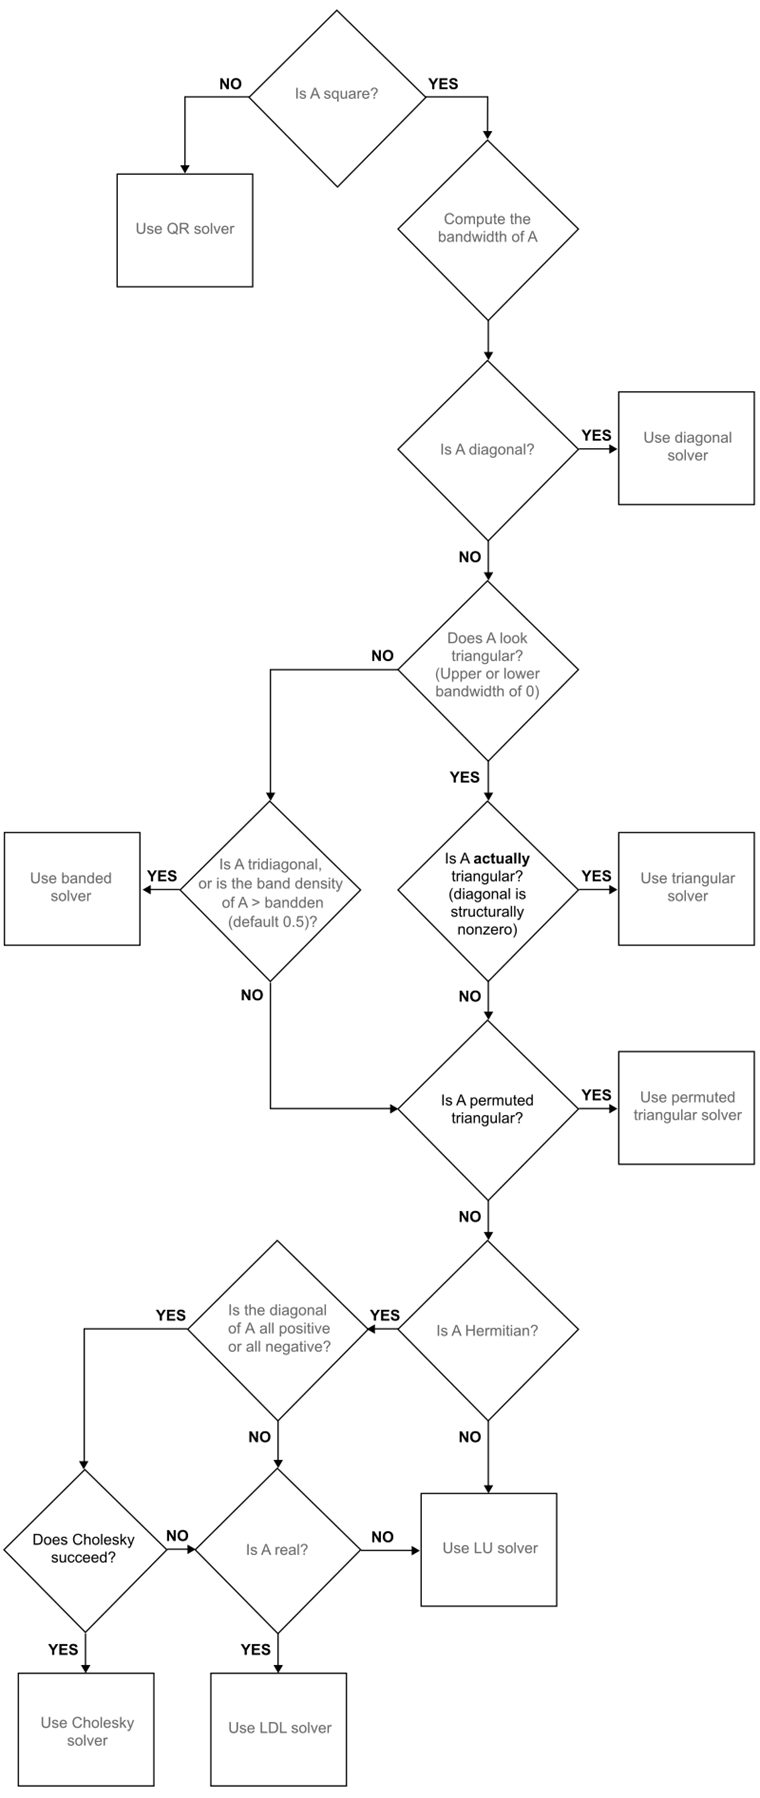
\includegraphics[width=.3\paperwidth]{mldivide_sparse}
              \caption{Diagrama de flujo del solucionador
                  \mintinline{octave}|mldivide| para matrices
                  disperas que emplea MATLAB.
                  Recuperado de~\url{https://www.mathworks.com/help/matlab/ref/double.mldivide.html}.}
          \end{figure}
\end{itemize}

\section*{Resultados del Programa~\ref{code:elliptic1D.m}}

En primer lugar, mostramos la gráfica a escala 1:1 de la solución
exacta y de la solución mimética obtenida en el Programa~\ref{code:elliptic1D.m}.

\begin{figure}[ht!]
    \centering
    % \includegraphics[width=.6\paperwidth]{../examples/octave/elliptic1D.pdf}
    \includegraphics[width=.39\paperwidth]{elliptic1D.pdf}
    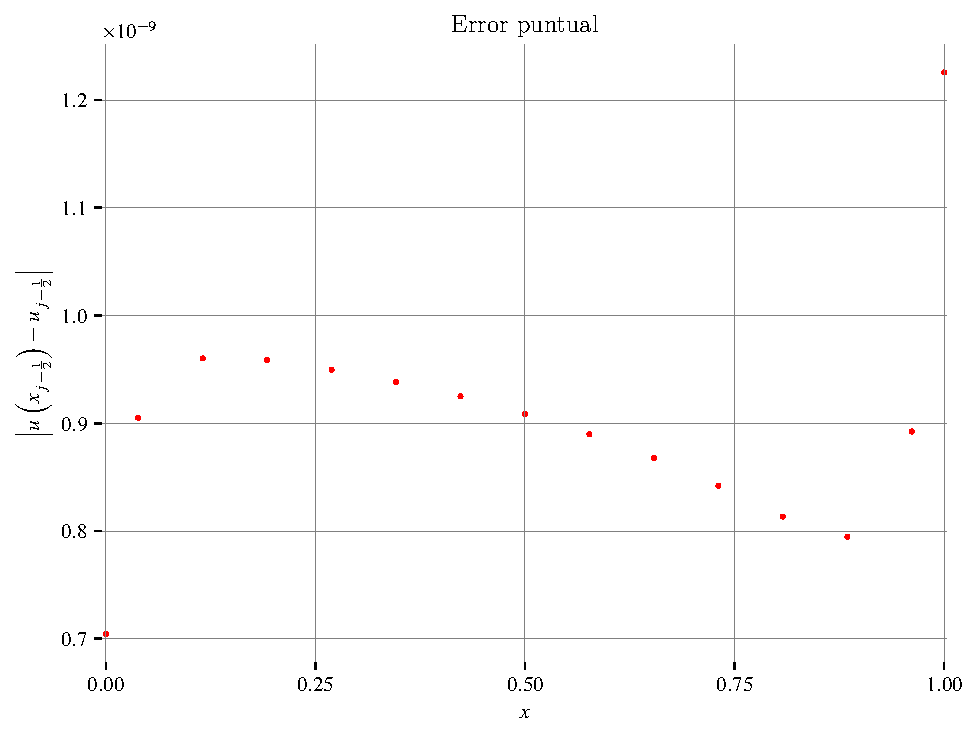
\includegraphics[width=.39\paperwidth]{elliptic1Derror.pdf}
    \caption{Izquierda: Solución de~\eqref{eq:poisson1drobindconditions}
        usando \mintinline{octave}|k=6| y \mintinline{octave}|m=2k+1=13|.
        Derecha: Error en la malla escalonada
        \begin{math}
            \left\{
            0,
            \dotsc,
            x_{j-\frac{1}{2}}
            \dotsc,
            1
            \right\}
        \end{math}}
\end{figure}

En segundo lugar, mostramos una gráfica del error en cada punto de la malla computacional
dada por
\begin{equation*}
    \text{Error de $u$ en $x_{j-\frac{1}{2}}$}=
    \left|
    u\left(x_{j-\frac{1}{2}}\right)-
    u_{j-\frac{1}{2}}
    \right|.
\end{equation*}

Por último, mostramos la tabla de los errores y el orden de convergencia numérico.

\begin{table}[ht!]
    \centering
    \begin{tabular}{ccc}
        \toprule
        $\Delta x$            & Error $\ell_1$        & Orden    \\
        \midrule
        $1.562\times 10^{-2}$ & $4.410\times 10^{-2}$ & -        \\
        $1.535\times 10^{-2}$ & $4.464\times 10^{-2}$ & $-0.678$ \\
        \bottomrule
    \end{tabular}
    \caption{Tabla de errores de aproximación de $U$ en
        $x_{j-\frac{1}{2}}$ y el orden convergencia numérico obtenido.}
    \label{table:errors}
\end{table}


\section{The 1D Diffusion Equation}

Given the one-dimensional heat equation

\begin{equation}\label{eq:IBVPheat1d}
    \begin{cases}
        \diffp{u}{t}=
        \kappa\diffp[2]{u}{x},
                                      & \left(x,t\right)\in
        \left(a,b \right)\times\left(0, \infty \right).     \\
        u\left(x,0\right)=f(x),
                                      & x\in
        \left[a,b\right].                                   \\
        u\left(a,t\right)= \alpha(t), & t\in
        \left(0,\infty\right),                              \\
        u\left(b,t\right)= \beta(t),
                                      & t\in
        \left(0,\infty\right),
    \end{cases}
\end{equation}

where $\kappa$ is the thermal diffusivity.\\

The 1D heat equation code by mimetic methods


\begin{listing}[ht!]
    \tiny
    \centering
    \pathinputminted[frame=single,framesep=12pt,linenos,firstline=1,lastline=80,highlightlines={20,29}]{octave}{parabolic1D.m}
    \caption{Programa~\texttt{parabolic1D.m}}
    \label{code:parabolic1D.m}
\end{listing}


In the one-dimensional heat equation in the parabolic1D.m code, the PDE being solved is given by:


\begin{equation}\label{eq:IBVPheat1d}
    \begin{cases}
        \diffp{u}{t}=
        \kappa\diffp[2]{u}{x},
                                 & \left(x,t\right)\in
        \left(0,1 \right)\times\left(0, 1 \right).     \\
        u\left(x,0\right)= 0,
                                 & x\in
        \left[0,1\right].                              \\
        u\left(0,t\right)= 100., & t\in
        \left(0,1 \right),                             \\
        u\left(1,t\right)= 100.,
                                 & t\in
        \left(0, 1\right),
    \end{cases}
\end{equation}


\textbf{Line 9:} In this part the code defines the value of the diffusion coefficient $\kappa =1$.\\

\textbf{Line 10:} Define the left side $a= 0$ of the domain of the variable $x$.\\

\textbf{Line 11:} Define the right hand side $b= 1$ of the domain of the variable $x$.\\

\textbf{Line 13:} The Operator's order of accuracy $k = 2$.\\

\textbf{Line 14:} $m$ is the number of cells, where $m$ can take values ​​$m \geq 2*k+1$; in this case $m=2*(2)+1=5$.\\

\textbf{Line 15:} In this line the step size in $x$ is defined, defined as $dx=(b-a)/m$, en this case, replacing it, we have $dx =\frac{1-0}{5} =\frac{1}{5}$ \\

\textbf{Line 17:} End time $t=1$.\\

\textbf{Line 18:} Von Neumann stability criterion for $k=2$, we have $ dt = \frac{(dx)^{2}}{3 \kappa}$, in this exercise the step in time is given by: $dt =\frac{1}{75}$\\

\textbf{Line 20:} $L = lap(k,m,dx)$ 1D mimetic Laplacian operator is of order $m+2$ so $m+2$ for this exercise is of order 7 by 7, where $k=2$, $m = 5$ and $\frac{1}{5}$, then $L = lap(2,5,\frac{1}{5})$.\\

\textbf{Line 23:} The initial condition  value $u(x,0)=0$ is a matrix of order $m+2$ by $1$, in this case $7$ by $1$.\\

\textbf{Line 25:} The boundary condition is on the left side u(a,t)= u(0,t)=100\\

\textbf{Line 26:} The boundary condition on the right side u(b,t)= u(1,t)=100\\

\textbf{Line 29:} The mesh used in the mimetic method  grid = $[west$  $west+dx/2: dx :east-dx/2$  $east]$, then grid = $[a$ $a+\frac{dx}{2}: dx : b-\frac{dx}{2}$ $b  ]$, in this exercise the mesh is given by:

\begin{center}

    grid = $[0$ $\frac{1}{10}: \frac{1}{5}: \frac{9}{10}$ $1]$ = $  \{0, \frac{1}{10}, \frac{3}{10}, \frac{5}{10}, \frac{7}{10}, \frac{9}{10}, 1 \}$

\end{center}

\textbf{Line 31:} If explicit=1 then the PDE will be solved in time by the explicit method, and if explicit=0 then the PDE will be solved by the implicit method.\\

\textbf{Line 33 to 50:} In this section we have the explicita solution of the PDE and the graph. \\

\textbf{Line 36:} The value of L is obtained by:

\begin{equation}
    \frac{\partial u}{\partial t} = \kappa \frac{\partial^{2} u}{\partial x^{2}}
\end{equation}

Discretizing $\frac{\partial u}{\partial t}$ by forward finite differences, and $\frac{\partial^{2} u}{\partial x^{2}}$ by applying mimetic methods

\begin{equation}
    \frac{u^{n+1}_{i} - u^{n}_{i} }{dt} = \kappa L 	u^{n}_{i}
\end{equation}

then clearing $u^{n+1}_{i}$ we obtain:


\begin{equation}
    u^{n+1}_{i} = u^{n}_{i}  +  \kappa dt L u^{n}_{i}
\end{equation}

Factoring $u^{n}_{i}$ we have:

\begin{equation}
    u^{n+1}_{i} = (I  +  \kappa dt L )u^{n}_{i}
\end{equation}

where $I$ is the identity matrix of general order $m+2$ by $m+2$, for this exercise of order $7$ by $7$, being

$$  L = (\kappa dt L +I )$$

being in the code: $ L = alpha*dt*L + speye(size(L))$; finally to obtain the solution

\begin{equation}
    u^{n+1}_{i} = L *u^{n}_{i}
\end{equation}

in the code on line 47 we have $ U = L*U.$\\


\textbf{Line 39:} The iteration starts for $t=0$ until $t=t/dt+1$, in this exercise $t/dt+1= 75+1=76$.\\


\textbf{Line 40 and 60:} The graph of the mesh on the $x$ axis by grid and the solution of the PDE $U$. \\


\textbf{Line 41 and 62:} In this line the graph is on the $x$ axis from 0 to 1 and on the $y$ axis from 0 to 105.\\


\textbf{Line 42 and 63:} In this line prints the different times ($ i* dt$)for explicit method, with two decimal  ($ .2f $).\\


\textbf{Line 43 and 64:} Use the title command to display the title designated on line 42. \\


\textbf{Line 44 and 65:} Label the $x$-axis in this exercise as $x$.


\textbf{Line 45 and 66:} Label the $y$-axis in this exercise as $T$.\\


\textbf{Line 46 and 67:} Shows the graph for the different times with a pause of 0.01. \\


\textbf{Line 50 to 71:} In this section we have the implicita solution of the PDE and the graph. \\

\textbf{Line 53:} The value of L is obtained by:

\begin{equation}
    \frac{\partial u}{\partial t} = \kappa \frac{\partial^{2} u}{\partial x^{2}}
\end{equation}

Discretizing $\frac{\partial u}{\partial t}$ by forward finite differences, and $\frac{\partial^{2} u}{\partial x^{2}}$ by applying mimetic methods

\begin{equation}
    \frac{u^{n+1}_{i} - u^{n}_{i} }{dt} = \kappa L 	u^{n+1}_{i}
\end{equation}

then clearing $u^{n+1}_{i}$ we obtain:


\begin{equation}
    u^{n+1}_{i}(I - \kappa dt L ) = u^{n}_{i}
\end{equation}

where $I$ is the identity matrix of general order $m+2$ by $m+2$, for this exercise of order $7$ by $7$, being

$$  L = (-\kappa dt L + I)$$

being in the code: $ L = -alpha*dt*L +speye(size(L))$.\\

\textbf{Line 54:} In this line $dL=$ decomputation($L$) the matrix L is decomposed into lower triangular matrix $L$ and upper triangular matrix $U$ using LU decomposition method.\\

\textbf{Line 68:} In this line solve the $u^{n+1} =(dL)^{-1}*u^{n}$, thus finding the solution $U=dL \setminus U$.\\



\section{Convection-diffusion}
Given the three-dimensional convection diffusion equation

\begin{equation}\label{eq:IBVP3d}
    \begin{cases}
        \diffp{u}{t} + \nabla(v u) = \nabla \cdot (D \nabla u),
                                      & \left(x,y,z,t\right)\in
        \left(a,b \right)\times\left(c,d \right)\times \left(e,f \right)\times\left(0, \infty \right).     \\
        u\left(x,0\right)=f(x),
                                      & x\in
        \left[a,b\right].                                   \\
        u\left(a,t\right)= \alpha(t), & t\in
        \left(0,\infty\right),                              \\
        u\left(b,t\right)= \beta(t),
                                      & t\in
        \left(0,\infty\right),
    \end{cases}
\end{equation}


\begin{listing}[ht!]
    \tiny
    \centering
    \pathinputminted[frame=single,framesep=12pt,linenos,firstline=1,lastline=80,highlightlines={20,29}]{octave}{convection_diffusion.m}
    \caption{Programa~\texttt{convection\_diffusion.m}}
    \label{code:convection_diffusion.m}
\end{listing}

\chapter{MOLE Tests}

\section{Test $1$}

\begin{listing}[ht!]
	\tiny
	\centering
	\pathinputminted[frame=single,framesep=10pt,linenos,firstline=1,lastline=33,highlightlines={9-19}]{cpp}{test1.cpp}
	\caption{Program~\texttt{test1.cpp}}
	\label{code:test1.cpp}
\end{listing}

\begin{listing}[ht!]
	\tiny
	\centering
	\pathinputminted[frame=single,framesep=10pt,linenos,firstline=1,lastline=21,highlightlines={8-19}]{octave}{test1.m}
	\caption{Program~\texttt{test1.m}}
	\label{code:test1.m}
\end{listing}

\section{Test $2$}

\begin{listing}[ht!]
	\tiny
	\centering
	\pathinputminted[frame=single,framesep=10pt,linenos,firstline=1,lastline=28,highlightlines={9-20}]{cpp}{test2.cpp}
	\caption{Program~\texttt{test2.cpp}}
	\label{code:test2.cpp}
\end{listing}

\begin{listing}[ht!]
	\tiny
	\centering
	\pathinputminted[frame=single,framesep=10pt,linenos,firstline=1,lastline=21,highlightlines={8-19}]{octave}{test2.m}
	\caption{Program~\texttt{test2.m}}
	\label{code:test2.m}
\end{listing}

\section{Test $3$}

\begin{listing}[ht!]
	\tiny
	\centering
	\pathinputminted[frame=single,framesep=10pt,linenos,firstline=1,lastline=27,highlightlines={8-19}]{cpp}{test3.cpp}
	\caption{Program~\texttt{test3.cpp}}
	\label{code:test3.cpp}
\end{listing}

\begin{listing}[ht!]
	\tiny
	\centering
	\pathinputminted[frame=single,framesep=10pt,linenos,firstline=1,lastline=21,highlightlines={8-19}]{octave}{test3.m}
	\caption{Program~\texttt{test3.m}}
	\label{code:test3.m}
\end{listing}

\section{Test $4$}

\begin{listing}[ht!]
	\tiny
	\centering
	\pathinputminted[frame=single,framesep=10pt,linenos,firstline=1,lastline=39,highlightlines={10-39}]{cpp}{test4.cpp}
	\caption{Program~\texttt{test4.cpp}}
	\label{code:test4.cpp}
\end{listing}

\begin{listing}[ht!]
	\tiny
	\centering
	\pathinputminted[frame=single,framesep=10pt,linenos,firstline=1,lastline=48,highlightlines={15-44}]{octave}{test4.m}
	\caption{Program~\texttt{test4.m}}
	\label{code:test4.m}
\end{listing}

\section{Test $5$}

\begin{listing}[ht!]
	\tiny
	\centering
	\pathinputminted[frame=single,framesep=10pt,linenos,firstline=1,lastline=61,highlightlines={9-53}]{cpp}{test5.cpp}
	\caption{Program~\texttt{test5.cpp}}
	\label{code:test5.cpp}
\end{listing}

\begin{listing}[ht!]
	\tiny
	\centering
	\pathinputminted[frame=single,framesep=10pt,linenos,firstline=1,lastline=55,highlightlines={10-53}]{octave}{test5.m}
	\caption{Program~\texttt{test5.m}}
	\label{code:test5.m}
\end{listing}

\part{Validation and Test Cases}

% TODO: Comparar algunas soluciones con el método de diferencias finitas, como por ejemplo, para la ecuación de onda.
% TODO: Ejemplo, donde el método numérico es conservativo (se conserva la energía)
\chapter{Operator Validation}

\section{Divergence Operator Tests}

\subsection{Test 1: Accuracy in 1D}
\subsection{Test 2: Conservation in 2D}
\subsection{Test 3: Boundary Compliance in 3D}
\section{Gradient and Laplacian Tests}
\section{Interpolation Robustness Checks}
\section{Application-Driven Tests}
\subsection{Stability Analysis for PDE Solvers}
\subsection{Performance Benchmarking}

MOLE uses \href{https://google.github.io/googletest}{GoogleTest} framework.

\begin{listing}[ht!]
	\tiny
	\centering
	\pathinputminted[frame=single,framesep=10pt,linenos,firstline=1,lastline=33,highlightlines={9-19}]{cpp}{test1.cpp}
	\caption{Program~\texttt{test1.cpp}}
	\label{code:test1.cpp}
\end{listing}

\begin{listing}[ht!]
	\tiny
	\centering
	\pathinputminted[frame=single,framesep=10pt,linenos,firstline=1,lastline=21,highlightlines={8-19}]{octave}{test1.m}
	\caption{Program~\texttt{test1.m}}
	\label{code:test1.m}
\end{listing}

\begin{listing}[ht!]
	\tiny
	\centering
	\pathinputminted[frame=single,framesep=10pt,linenos,firstline=1,lastline=28,highlightlines={9-20}]{cpp}{test2.cpp}
	\caption{Program~\texttt{test2.cpp}}
	\label{code:test2.cpp}
\end{listing}

\begin{listing}[ht!]
	\tiny
	\centering
	\pathinputminted[frame=single,framesep=10pt,linenos,firstline=1,lastline=21,highlightlines={8-19}]{octave}{test2.m}
	\caption{Program~\texttt{test2.m}}
	\label{code:test2.m}
\end{listing}

\begin{listing}[ht!]
	\tiny
	\centering
	\pathinputminted[frame=single,framesep=10pt,linenos,firstline=1,lastline=27,highlightlines={8-19}]{cpp}{test3.cpp}
	\caption{Program~\texttt{test3.cpp}}
	\label{code:test3.cpp}
\end{listing}

\begin{listing}[ht!]
	\tiny
	\centering
	\pathinputminted[frame=single,framesep=10pt,linenos,firstline=1,lastline=21,highlightlines={8-19}]{octave}{test3.m}
	\caption{Program~\texttt{test3.m}}
	\label{code:test3.m}
\end{listing}

\begin{listing}[ht!]
	\tiny
	\centering
	\pathinputminted[frame=single,framesep=10pt,linenos,firstline=1,lastline=39,highlightlines={10-39}]{cpp}{test4.cpp}
	\caption{Program~\texttt{test4.cpp}}
	\label{code:test4.cpp}
\end{listing}

\begin{listing}[ht!]
	\tiny
	\centering
	\pathinputminted[frame=single,framesep=10pt,linenos,firstline=1,lastline=48,highlightlines={15-44}]{octave}{test4.m}
	\caption{Program~\texttt{test4.m}}
	\label{code:test4.m}
\end{listing}

\begin{listing}[ht!]
	\tiny
	\centering
	\pathinputminted[frame=single,framesep=10pt,linenos,firstline=1,lastline=61,highlightlines={9-53}]{cpp}{test5.cpp}
	\caption{Program~\texttt{test5.cpp}}
	\label{code:test5.cpp}
\end{listing}

\begin{listing}[ht!]
	\tiny
	\centering
	\pathinputminted[frame=single,framesep=10pt,linenos,firstline=1,lastline=55,highlightlines={10-53}]{octave}{test5.m}
	\caption{Program~\texttt{test5.m}}
	\label{code:test5.m}
\end{listing}




\appendix

\chapter{Installation Guides}

To work through this tutorial requires to have a working installation
of MOLE.
It relies on
\href{https://gitlab.com/conradsnicta/armadillo-code}{\mintinline{cpp}|armadillo|}~\cite{Sanderson2025},
a C++ library that provides data structures for sparse matrices.
We explain the step-by-step process for
\href{https://wiki.archlinux.org/title/Pacman/Rosetta}{Arch Linux}
and \href{https://help.ubuntu.com/lts/ubuntu-help/index.html}{Ubuntu Linux},
as both systems have been successfully tested by us.
% We believe that the best choice for getting started in scientific computing is GNU/Linux.
% \href{https://books.goalkicker.com/LinuxBook}{Linux commands Notes for Professionals book}.

\section{GNU/Linux (Arch, Ubuntu)}

This distribution is supported by a proactive group of
\href{https://archlinux.org/people/developers}{developers},
\href{https://archlinux.org/people/package-maintainers}{package maintainers}
and \href{https://archlinux.org/people/support-staff}{support staff}
that try to provide the latest stable software releases.
The steps are outlined in the Program~\ref{code:installerarchlinux.sh}.

\begin{listing}[ht!]
	\tiny
	\centering
	\pathinputminted[frame=single,framesep=10pt,linenos,firstline=1,lastline=18,highlightlines={9,15},escapeinside=||]{bash}{installerarchlinux.sh}
	\caption{Steps for a system-wide installation both C++ and Octave
		MOLE library via
		\href{https://raw.githubusercontent.com/carlosal1015/mole_examples/main/tutorial/installerarchlinux.sh}{\texttt{installerarchlinux.sh}}.}
	\label{code:installerarchlinux.sh}
\end{listing}

Even if you are using Windows, the
\href{https://docs.docker.com/desktop/features/wsl}{Docker Desktop WSL 2 backend}
is ideal for using MOLE via Program~\ref{code:docker.sh} or
\href{https://wiki.archlinux.org/title/Install_Arch_Linux_on_WSL}{installing Arch Linux on WSL 2} and following
the Program~\ref{code:installerarchlinux.sh}.

\begin{listing}[ht!]
	\tiny
	\centering
	\pathinputminted[frame=single,framesep=10pt,linenos,firstline=1,lastline=7,highlightlines={3}]{bash}{docker.sh}
	\caption{Pull container based on Arch Linux with set up MOLE
		library via \href{https://raw.githubusercontent.com/carlosal1015/mole_examples/main/tutorial/docker.sh}{\texttt{docker.sh}}.}
	\label{code:docker.sh}
\end{listing}

% \section{MOLE on Ubuntu Linux}

This \href{https://www.debian.org}{Debian}-derived distribution is
managed by \href{https://canonical.com}{Canonical Ltd.}
Each 2 years they launch a Long Term Support(LTS) release.
The steps are outlined in the Program~\ref{code:installerubuntu.sh}.

\begin{listing}[ht!]
	\tiny
	\centering
	\pathinputminted[frame=single,framesep=10pt,linenos,firstline=1,lastline=25,highlightlines={9,15}]{bash}{installerubuntu.sh}
	\caption{Steps for a system-wide installation both C++ and Octave
		MOLE library vía \href{https://raw.githubusercontent.com/carlosal1015/mole_examples/main/tutorial/installerubuntu.sh}{\texttt{installerubuntu.sh}}.}
	\label{code:installerubuntu.sh}
\end{listing}

\chapter{MOLE Documentation}

\section{Mimetic Operator's Library Enhanced Reference}

We split the MOLE documentation in three categories:

\begin{description}
	\item[\href{https://carlosal1015.github.io/mole_examples/html}{General MOLE documentation}]

	      It contains general information and examples.

	\item[\href{https://carlosal1015.github.io/mole_examples/doxygen/cpp/html}{C++ MOLE documentation}]

	      It contains API C++ Reference.

	\item[\href{https://carlosal1015.github.io/mole_examples/doxygen/matlab}{Octave MOLE documentation}]

	      It contains API GNU/Octave Reference.
\end{description}

\section{Programming languages documentation}

\begin{description}
	\item[\href{https://en.cppreference.com}{C++ docs}]

	      \mintinline{cpp}|#include <iostream>|

	      \mintinline{cpp}|#include <cmath>|

	      \mintinline{cpp}|#include <vector>|.

	\item[\href{https://docs.octave.org}{Octave docs}]

	      \mintinline{octave}|addpath("/usr/share/")|.

	\item[\href{https://www.mathworks.com/help/matlab/index.html}{MATLAB docs}]

	      .
\end{description}

\section{Linear Algebra software documentation}

\begin{description}
	\item[\href{https://www.intel.com/content/www/us/en/developer/tools/oneapi/onemkl-documentation.html}{Intel MKL docs}]

	      .

	\item[\href{http://www.openmathlib.org/OpenBLAS/docs}{Openblas docs}]

	      .

	\item[\href{https://www.netlib.org/lapack/explore-html}{Netlib Lapack docs}]

	      .

	\item[\href{https://portal.nersc.gov/project/sparse/superlu/superlu_code_html/index.html}{SuperLU docs}]

	      .

	\item[\href{https://eigen.tuxfamily.org/dox}{Eigen docs}]

	      .

	\item[\href{https://arma.sourceforge.net/docs.html}{Armadillo docs}]

	      .
\end{description}

\begin{description}
	\item[\href{https://google.github.io/googletest}{Gtest docs}]

	      .

	\item[\href{https://docs.scipy.org/doc/scipy/reference/sparse.html}{SciPy sparse docs}]

	      .

	\item[\href{https://matplotlib.org/stable/api/_as_gen/matplotlib.pyplot.plot.html}{Matplotlib docs}]

	      .

	\item[\href{https://docs.h5py.org/en/stable}{HDF5 for Python docs}]

	      .
\end{description}

\chapter{Sparse Linear Algebra software examples}

\section{Armadillo}

We follow this gentle
\href{https://anderkve.github.io/FYS3150/book/introduction_to_cpp/intro_to_armadillo.html}{\emph{Introduction to Armadillo}}.

\subsection{Vectors}

\begin{listing}[ht!]
	\tiny
	\centering
	\pathinputminted[frame=single,framesep=12pt,linenos,firstline=1,lastline=56,highlightlines={43-44}]{cpp}{1.cc}
	\caption{Program~\texttt{1.cc}}
	\label{code:1.m}
\end{listing}

\subsection{Matrices}

\subsubsection{Dense Matrices}

\subsubsection{Sparse Matrices}

\subsubsection{Solvers}

\section{Eigen}

\section{SciPy Sparse}

See \href{https://github.com/nutrik/pymole}{pymole}.

\section{Sparse Arrays Julia}

See \href{https://robertsweeneyblanco.github.io/Programming_for_Mathematical_Applications/content/Sparse_Matrices/Sparse_Matrices_In_Julia.html}{}

\section{Fortran Sparse}

% https://www.intel.com/content/www/us/en/docs/onemkl/developer-reference-fortran/2024-0/inspector-executor-sparse-blas-routines.html
\section{Sparse Linear Algebra in Rust}

%https://github.com/sparsemat/sprs
%https://www.nalgebra.org

\section{PETSc sparse matrices in C}


\chapter{Supplementary Methods}

\section{Vector Calculus}

Vector Fields are maps of the form
\begin{equation*}
	F\colon\mathbb{R}^{n}\to\mathbb{R}^{n}
\end{equation*}
Scalar fields are maps of the form
\begin{equation*}
	\phi\colon\mathbb{R}^{n}\to\mathbb{R}
\end{equation*}
The gradient of a scalar field is a vector field, defined as
\begin{equation*}
	\nabla\phi=
	\diffp{\phi}{x^{i}}\symbf{e}_{i}
\end{equation*}
Given Cartesian coordinates $x^{i}$ with $i=1,\dotsc,n$ on $\mathbb{R}^{n}$,
the gradient of $\phi$ is defined as
\begin{equation*}
	\nabla\phi=
	\diffp{\phi}{x^{i}}\symbf{e}_{i}.
\end{equation*}
A vector field $\symbf{F}$ is called conservative if it can be written as
\begin{equation*}
	\symbf{F}=\nabla\phi.
\end{equation*}
Given two vectors, a derivative acting on vector fields known as the divergence
\begin{equation*}
	\nabla\cdot\symbf{F}=
	\left(\symbf{e}_{i}\diffp{}{x^{i}}\right)\cdot
	\left(\symbf{e}_{j}F_{j}\right)=
	\diffp{F_{i}}{x^{i}}
\end{equation*}
where $\symbf{e}_{i}\cdot\symbf{e}_{j}=\delta_{ij}$.
Note that the gradient of a scalar filed gave a vector field.
Now the divergence of a vector field gives a scalar field.
If $\symbf{F}\colon\mathbb{R}^{3}\to\mathbb{R}^{3}$, we can take cross product.
\begin{equation*}
	\nabla\times\symbf{F}=
	\left(\right)\times\left(\right)=
	\epsilon_{ijk}\diffp{F_{j}}{x^{i}}\symbf{e}_{k}
\end{equation*}

\begin{equation*}
	\nabla\times\symbf{F}=
	\left(
	\diffp{F_{3}}{x^{2}}-\diffp{F_{2}}{x^{3}},
	\diffp{F_{1}}{x^{3}}-\diffp{F_{3}}{x^{1}},
	\diffp{F_{2}}{x^{1}}-\diffp{F_{1}}{x^{2}}
	\right)=
	\begin{vmatrix}
		\symbf{e}_{1}   & \symbf{e}_{2}   & \symbf{e}_{3}   \\
		\diffp{}{x^{1}} & \diffp{}{x^{2}} & \diffp{}{x^{3}} \\
		F_{1}           & F_{2}           & F_{3}
	\end{vmatrix}
\end{equation*}

\begin{align*}
	\nabla\left(\alpha\phi+\psi\right)                 & =
	\alpha\nabla\phi+\nabla\psi.                           \\
	\nabla\cdot\left(\alpha\symbf{F}+\symbf{G}\right)  & =
	\alpha\nabla\cdot\symbf{F}+\nabla\cdot\symbf{G}.       \\
	\nabla\times\left(\alpha\symbf{F}+\symbf{G}\right) & =
	\alpha\nabla\times\symbf{F}+\nabla\times\symbf{G}.
\end{align*}
for any scalar fields $\phi$ and $\psi$, vector fields $\symbf{F}$ and $\symbf{G}$,
and any constant $\alpha$.

\begin{align*}
	\nabla\left(\phi\psi\right)            & =
	\phi\nabla\psi+\psi\nabla\phi.                                              \\
	\nabla\cdot\left(\phi\symbf{F}\right)  & =
	\left(\nabla\phi\right)\cdot\symbf{F}+\phi\left(\nabla\cdot\symbf{F}\right) \\
	\nabla\times\left(\phi\symbf{F}\right) & =
	\left(\nabla\phi\right)\times\symbf{F}+\phi\left(\nabla\times\symbf{F}\right)
\end{align*}

\begin{equation*}
	\nabla\cdot\left(\phi\symbf{F}\right)=
	\diffp{\left(\phi F_{i}\right)}{x^{i}}=
	\diffp{\phi}{x^{i}}F_{i}+
	\phi\diffp{F_{i}}{x^{i}}=
	\left(\nabla\phi\right)\cdot\symbf{F}+
	\phi\left(\nabla\cdot\symbf{F}\right).
\end{equation*}

\begin{equation*}
	\nabla\cdot\left(F\times G\right)=
	\left(\nabla\times\symbf{F}\right)\cdot\symbf{G}-
	\symbf{F}\cdot\left(\nabla\times\symbf{G}\right).
\end{equation*}

\begin{equation*}
	\symbf{F}\cdot\nabla=F_{i}\diffp{}{x^{i}}
\end{equation*}
\begin{equation*}
	\symbf{F}\times\nabla=
	\symbf{e}_{k}
	\epsilon_{ijk}
	F_{i}\diffp{}{x^{j}}
\end{equation*}

\begin{align*}
	\nabla\left(\symbf{F}\cdot\symbf{G}\right)        & =
	\symbf{F}\times\left(\nabla\times\symbf{G}\right)+
	\symbf{G}\times\left(\nabla\times\symbf{F}\right)+
	\left(\symbf{F}\cdot\nabla\right)\symbf{G}+
	\left(\symbf{G}\cdot\nabla\right)\symbf{F}.           \\
	\nabla\times\left(\symbf{F}\times\symbf{G}\right) & =
	\left(\nabla\cdot\symbf{G}\right)\symbf{F}-
	\left(\nabla\cdot\symbf{F}\right)\symbf{G}+
	\left(\symbf{G}\cdot\nabla\right)\symbf{F}-
	\left(\symbf{F}\cdot\nabla\right)\symbf{G}.
\end{align*}

\begin{equation*}
	\nabla\times\symbf{F}=
	0\iff
	\symbf{F}=
	\nabla\phi\iff
	\oint_{C}
	\symbf{F}\cdot\dl{\symbf{x}}=
	0.
\end{equation*}

\begin{equation*}
	\nabla\cdot\symbf{F}=0\iff
	\symbf{F}=\nabla\times\symbf{A}.
\end{equation*}

The Laplacian is a second order differential operator defined by
\begin{equation*}
	\nabla^{2}=
	\nabla\cdot\nabla=
	\diff[2]{}{x^{i},x^{i}}
\end{equation*}

\begin{equation*}
	\nabla^{2}=
	\diffp[2]{}{x}+
	\diffp[2]{}{y}+
	\diffp[2]{}{z}.
\end{equation*}

\begin{equation*}
	\nabla\times\left(\nabla\times\symbf{F}\right)=
	\nabla\left(\nabla\cdot\symbf{F}\right)-\nabla^{2}\symbf{F}.
\end{equation*}

\begin{equation*}
	\nabla^{2}\symbf{F}=
	\nabla\left(\nabla\cdot\symbf{F}\right)-\nabla\times\left(\nabla\times\symbf{F}\right)
\end{equation*}

\begin{align*}
	\nabla\cdot\symbf{E}  & =\frac{\rho}{\epsilon_{0}} \\
	\nabla\times\symbf{E} & =-\diffp{\symbf{B}}{t}     \\
	\nabla\cdot\symbf{B}  & =0                         \\
	\nabla\times\symbf{B}=
	\mu_{0}\left(\symbf{J}+\epsilon_{0}\diffp{\symbf{E}}{t}\right)
\end{align*}

\begin{equation*}
	\dl f=
	\diffp{f}{u}\dl u+
	\diffp{f}{v}\dl v+
	\diffp{f}{w}\dl w=
	\nabla f\cdot
	\left(
	h_{u}\symbf{e}_{u}\dl u+
	h_{v}\symbf{e}_{v}\dl v+
	h_{w}\symbf{e}_{w}\dl w
	\right)
\end{equation*}

\begin{equation*}
	\nabla=
	\frac{1}{h_{u}}\symbf{e}_{u}\diffp{}{u}+
	\frac{1}{h_{v}}\symbf{e}_{v}\diffp{}{v}+
	\frac{1}{h_{w}}\symbf{e}_{w}\diffp{}{w}
\end{equation*}

\begin{equation*}
	F\left(u,v,w\right)=
	F_{u}\symbf{e}_{u}+
	F_{v}\symbf{e}_{v}+
	F_{w}\symbf{e}_{w}
\end{equation*}

\begin{equation*}
	\nabla\cdot\symbf{F}=
	\frac{1}{h_{u}h_{v}h_{w}}
	\left(
	\diffp{}{u}\left(h_{v}h_{w}F_{u}\right)+
	\diffp{}{v}\left(h_{u}h_{w}F_{v}\right)+
	\diffp{}{w}\left(h_{u}h_{v}F_{w}\right)
	\right)
\end{equation*}

\begin{equation*}
	\nabla\times\symbf{F}=
	\frac{1}{h_{u}h_{v}h_{w}}
	\begin{vmatrix}
		h_{u}\symbf{e}_{u} & h_{v}\symbf{e}_{v} & h_{w}\symbf{e}_{w} \\
		\diffp{}{u}        & \diffp{}{v}        & \diffp{}{w}        \\
		h_{u}F_{u}         & h_{v}F_{v}         & h_{w}F_{w}
	\end{vmatrix}
\end{equation*}

\begin{equation*}
	\nabla^{2}f=
	\nabla\cdot\nabla f=
	\frac{1}{h_{u}h_{v}h_{w}}
	\left[
		\diffp{}{u}\left(\frac{h_{v}h_{w}}{h_{u}}\diffp{f}{u}\right)+
		\diffp{}{v}\left(\frac{h_{u}h_{w}}{h_{v}}\diffp{f}{v}\right)+
		\diffp{}{w}\left(\frac{h_{u}h_{v}}{h_{w}}\diffp{f}{w}\right)
		\right]
\end{equation*}

\begin{equation*}
	\nabla^{2}f=
	\diffp[2]{f}{x}+
	\diffp[2]{f}{y}
	\diffp[2]{f}{z}.
\end{equation*}

\begin{equation*}
	\nabla^{2}f=
	\frac{1}{\rho}
	\diffp{}{\rho}
	\left(\rho\diffp{f}{\rho}\right)+
	\frac{1}{\rho^{2}}\diffp[2]{f}{\phi}+
	\diffp[2]{f}{z}.
\end{equation*}

\begin{equation*}
	\nabla^{2}f=
	\frac{1}{r^{2}}
	\diffp{}{r}\left(r^{2}\diffp{f}{r}\right)+
	\frac{1}{r^{2}\sin\theta}
	\diffp{}{\theta}
	\left(\sin\theta\diffp{f}{\theta}\right)+
	\frac{1}{r^{2}\sin^{2}\theta}
	\diffp[2]{f}{\phi}.
\end{equation*}

\subsection{The Divergence Theorem}

For a smooth vector field $\symbf{F}\left(\symbf{x}\right)$ over $\mathbb{R}^{3}$,
\begin{equation*}
	\int_{V}\nabla\cdot\symbf{F}\dl V=
	\int_{S}\symbf{F}\cdot\dl{\symbf{S}}
\end{equation*}
where $V$ is a bounded region whose boundary $\partial V=S$ is a piecewise smooth closed surface.
The integral on the right-hand side is taken with the normal $\symbf{n}$ pointing outward.

\begin{equation*}
	\int_{V}
	\nabla\cdot\symbf{F}\dl V\approx V\nabla\cdot\symbf{F}\left(\symbf{x}\right).
\end{equation*}

\begin{equation*}
	\nabla\cdot\symbf{F}=
	\lim_{V\to0}\frac{1}{V}\int_{S}\symbf{F}\cdot\dl{\symbf{S}}
\end{equation*}

\begin{equation*}
	\int_{S}
	\symbf{F}\cdot\dl{\symbf{S}}=
	\int_{V}\nabla\cdot\symbf{F}\dl V.
\end{equation*}

We introduce the density $\rho\left(\symbf{x},t\right)$ of the conserved object.
The total electric charge in some region $V$ is then given by the integral
\begin{equation*}
	Q=
	\int_{V}\rho\dl V.
\end{equation*}

The conservation of charge is captured by the following statement:
there exists a vector field $\symbf{J}\left(\symbf{x},t\right)$ such that
\begin{equation*}
	\diffp{\rho}{t}+
	\nabla\cdot\symbf{J}=0
\end{equation*}

This is known as the continuity equation and $\symbf{J}$ is called the current density.

\begin{equation*}
	\diffp{Q}{t}=
	\int_{V}
	\diffp{\rho}{t}\dl V=
	-\int_{V}\nabla\cdot\symbf{J}\dl V=
	-\int_{S}
	\symbf{J}\cdot\dl{\symbf{S}}.
\end{equation*}

The continuity equation plays an important role in Fluid Dynamics
where the mass is conserved.
In that case, $\rho\left(\symbf{x},t\right)$ is the density
of the fluid and the current is $\symbf{J}=\rho\symbf{u}$ where
$\symbf{u}\left(\symbf{x},t\right)$ is the velocity field.
The continuity equation then read as
\begin{equation*}
	\diffp{\rho}{t}+
	\nabla\cdot\left(\rho\symbf{u}\right)=0.
\end{equation*}

In many circumstances, liquids can be modelled as incompressible, meaning
that $\rho\left(\symbf{x},t\right)$ is a constant in both space and time.
In these circumstances, we have $\dot{\rho}=\nabla\rho=0$ and the
continuity equation tell us that the velocity field is necessarily solenoidal:
\begin{equation*}
	\nabla\cdot\symbf{u}=0
\end{equation*}

There is a close connection between conserved quantities and the idea of diffusion.
We will illustrate this with the idea of energy conservation.
The story takes slightly different from depending on the context, but here we will
think of the energy contained in a hot gas.
First, since energy is conserved there is necessarily a corresponding
continuity equation.
\begin{equation*}
	\diffp{\symbf{\mathcal{E}}}{t}+\nabla\cdot\symbf{J}=0
\end{equation*}
where $\symbf{\mathcal{E}}\left(\symbf{x},t\right)$ is the energy density of the gas,
and $\symbf{J}$ is the heat current which tell us how energy is transported from
one region of space to another.
First, the energy density in a gas is proportional to the temperature of the gas
\begin{equation*}
	\symbf{\mathcal{E}}\left(\symbf{x},t\right)=
	c_{V}T\left(\symbf{x},t\right)
\end{equation*}
where $c_{V}$ is the specific heat capacity.

\begin{equation*}
	\symbf{J}=-\kappa\nabla T
\end{equation*}
where $\kappa$ is called the thermal conductivity.
This relation is known as Fick's law.

Let $P\left(x,y\right)$ and $Q\left(x,y\right)$ be smooth functions on $\mathbb{R}^{2}$.
Then
\begin{equation*}
	\int_{A}\left(\diffp{Q}{x}-\diffp{P}{y}\right)\dl A=
	\oint_{C}
	\left(P\dl x+Q\dl y\right)
\end{equation*}
where $A$ is a bounded region in the plane and $C=\partial A$ is a piecewise smooth,
non-intersecting closed curve which is traversed anti-clockwise.

\subsection{The Stokes Theorem}

Stoke's theorem is an extension of Green's theorem, but where the surface is no
longer restricted to lie in a plane.

Let $S$ be a smooth surface in $\mathbb{R}^{3}$ with boundary $C=\partial S$ a piecewise
smooth curve.
For any smooth vector field $\symbf{F}\left(\symbf{x}\right)$, we have
\begin{equation*}
	\int_{S}
	\nabla\times\symbf{F}\cdot\dl{\symbf{S}}=
	\int_{C}
	\symbf{F}\cdot\dl{\symbf{x}}
\end{equation*}

\begin{equation*}
	\int_{S}
	\nabla\times\symbf{F}\cdot\dl{\symbf{S}}\approx
	A\symbf{n}\cdot\left(\nabla\times\symbf{F}\right).
\end{equation*}

\begin{equation*}
	\symbf{n}\cdot\left(\nabla\times\symbf{F}\right)=
	\lim_{A\to0}
	\int_{C}\symbf{F}\cdot\dl{\symbf{x}}.
\end{equation*}
In other words, at any given point, the value of $\nabla\times\symbf{F}$ in the direction $\symbf{n}$
tell us about the circulation of $\symbf{F}$ in the plane normal to $\symbf{n}$.

\begin{equation*}
	\nabla\times\symbf{F}=0\implies
	\oint_{C}\symbf{F}\cdot\dl{\symbf{x}}=0
\end{equation*}
for all closed curve $C$.

\subsection{Tensor Fields}

A tensor field over $\mathbb{R}^{3}$ is the assignment of a tensor $T_{i,\dotsc,k}\left(\symbf{x}\right)$
to every point $\symbf{x}\in\mathbb{R}^{3}$.
This is a generalization of a vector field
\begin{equation*}
	\symbf{F}\colon\mathbb{R}^{3}\to\mathbb{R}^{3}
\end{equation*}
to a map of the kind
\begin{equation*}
	T\colon\mathbb{R}^{3}\to\mathbb{R}^{m}
\end{equation*}
with $m$ the number of components of the tensor.

\section{Method of characteristics}

\cite{Choksi2022,Arrigo2023}

Let's consider the problem of

\begin{equation*}
	\begin{cases}
		\difcp{u}{t}+
		c\difcp{u}{x}=0,   & x\in\left(0,1\right),\, t>0. \\
		u\left(0,t\right)=
		u\left(1,t\right), & t>0.                         \\
		u\left(x,0\right)=
		g\left(x\right),   & x\in\left[0,1\right].
	\end{cases}
\end{equation*}

Consider the problem for the explicit form of linear first-oder
PDEs in two independent variables

\begin{equation*}
	\begin{cases}
		a
		\left(x,y\right)
		\difcp{u}{x}+
		b
		\left(x,y\right)
		\difcp{u}{y}=
		c_{1}
		\left(x,y\right)
		u+
		c_{2}
		\left(x,y\right), \\
		u\left(x,y\right)
		\text{given for}
		\left(x,y\right)\in
		\Gamma.
	\end{cases}
\end{equation*}

to be solved in some domain
\begin{math}
	\Omega\subset
	\mathbb{R}^{2}
\end{math}
with data given on some curve
\begin{math}
	\Gamma\subset
	\overline\Omega
\end{math}.

Often the
\begin{math}
	\Gamma\subset
	\partial\Omega\subset
	\mathbb{R}^{2}
\end{math}
it will just be one of the coordinate axes.

We find the characteristics, i.e., the curves which follow these
directions, by solving

\begin{equation*}
	\diff{x}{s}=
	a
	\left(
	x\left(s\right),
	y\left(s\right)
	\right),\qquad
	\diff{y}{s}=
	b
	\left(
	x\left(s\right),
	y\left(s\right)
	\right).
\end{equation*}

Now suppose $u$ is a solution to the PDE.
Let $z\left(s\right)$ denote the values of the solution $u$ along a
characteristic; i.e.,

\begin{equation*}
	z
	\left(s\right)\coloneqq
	u
	\left(
	x\left(s\right),
	y\left(s\right)
	\right).
\end{equation*}

Then by the chain rule, we have
\begin{align*}
	\diff{z}{s}
	 & =
	\difcp{u}{x}
	\left(
	x\left(s\right),
	y\left(s\right)
	\right)
	\diff{x}{s}
	\left(
	x\left(s\right),
	y\left(s\right)
	\right)+
	\difcp{u}{y}
	\left(
	x\left(s\right),
	y\left(s\right)
	\right)
	\diff{y}{s}
	\left(
	x\left(s\right),
	y\left(s\right)
	\right). \\
	\diff{z}{s}
	 & =
	\difcp{u}{x}
	\left(
	x\left(s\right),
	y\left(s\right)
	\right)
	a
	\left(
	x\left(s\right),
	y\left(s\right)
	\right)+
	\difcp{u}{y}
	\left(
	x\left(s\right),
	y\left(s\right)
	\right)
	b
	\left(
	x\left(s\right),
	y\left(s\right)
	\right). \\
	\diff{z}{s}
	 & =
	c_{1}
	\left(
	x\left(s\right),
	y\left(s\right)
	\right)
	z
	\left(s\right)+
	c_{2}
	\left(
	x\left(s\right),
	y\left(s\right)
	\right).
\end{align*}

\begin{definition}{Characteristics equations}{characteristics}
	There are three \emph{dependent variables} $x$, $y$ and $z$ and
	one \emph{independent} variable $s$.
	\begin{equation*}
		\begin{cases}
			\diff{x}{s}
			\left(s\right) & =
			a
			\left(
			x\left(s\right),
			y\left(s\right)
			\right).           \\
			\diff{y}{s}
			\left(s\right) & =
			b
			\left(
			x\left(s\right),
			y\left(s\right)
			\right).           \\
			\diff{z}{s}
			\left(s\right) & =
			c_{1}
			\left(
			x\left(s\right),
			y\left(s\right)
			\right)
			z
			\left(s\right)+
			c_{2}
			\left(
			x\left(s\right),
			y\left(s\right)
			\right).
		\end{cases}
	\end{equation*}
\end{definition}

\begin{figure}[ht!]
	\centering
	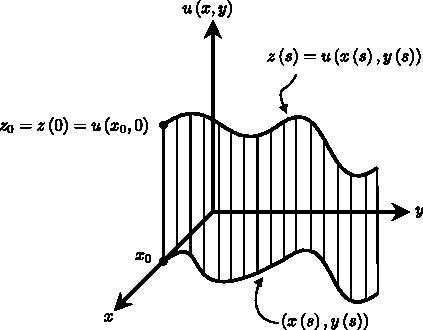
\includegraphics[width=0.35\paperwidth]{characteristics}
	\caption{The solution $u$ is described by the surface defined by
		$z=u\left(x,y\right)$.
		From any point $x_{0}$ on the $x$-axis, there is a curve
		$\left(x\left(s\right),y\left(s\right)\right)$ in the
		$xy$-plane, upon which wa can calculate the solution
		$z=u\left(x\left(s\right),y\left(s\right)\right)$.
		Knowing only the structure of the PDE, $x_{0}$ and $z_{0}$ we
		can solve ODEs to find the part of the solution surface which
		lies above the curve.}
\end{figure}

\begin{equation*}
	a\left(x,y\right)\diffp{u}{x}+
	b\left(x,y\right)\diffp{u}{y}=
	c_{1}\left(x,y\right)u+
	c_{2}\left(x,y\right),
	u\text{ given for }\left(x,y\right)\in\Gamma
\end{equation*}
where we have a linear PDE in the independent variables $x$ and $y$
with a given functions $a$, $b$, $c_{1}$ and $c_{2}$ of $\left(x,y\right)$.
$\Gamma\subset\partial\Omega$.
We find the characteristics, i.e., the curves which follow these directions, by solving
\begin{align*}
	\diff{x}{s}     & =
	a\left(x\left(s\right),y\left(s\right)\right). \\
	\diff{y}{s}     & =
	b\left(x\left(s\right),y\left(s\right)\right). \\
	z\left(s\right) & =
	u\left(x\left(s\right),y\left(s\right)\right).
\end{align*}

\begin{equation*}
	\diff{z}{s}=
	c_{1}\left(x\left(s\right),y\left(s\right)\right)
	z\left(s\right)+
	c_{2}\left(x\left(s\right),y\left(s\right)\right).
\end{equation*}

\section{Method of separation of variables}

\chapter{Code Repositories and Resources}

% https://sci-hub.se/10.1137/S0895479801398025

\backmatter
\nocite{*}
\printbibliography[title={References}]
\end{document}
